\documentclass[10pt,leqno]{amsart}
\usepackage{graphicx}
\usepackage{ifthen}
\usepackage{tikz}
\usepackage{eso-pic}
% \usepackage[margin=1in]{geometry}
%\usepackage{amsmath,amssymb}
\usepackage{hyperref}
\usepackage{color}
\usepackage{float}
\usepackage{multicol}
\usepackage{setspace}
\usepackage{mathptmx}
%\usepackage{mathpazo}
\usepackage[theorems]{tcolorbox}
\usepackage{mdframed}
\usepackage{amsmath,amsthm,amssymb,mathtools,flexisym,amsfonts,bbm}
\usepackage{xcolor,paralist,hyperref,fancyhdr,etoolbox}
\usepackage{mathrsfs}
\usepackage{booktabs}
\usepackage{pgfplots}
\usepackage{xcolor}
\usepackage[shortlabels]{enumitem}
\usepackage{algorithm}
\usepackage[noend]{algpseudocode}
\usepackage{cite}
\usepackage{multirow}
\usepackage[font=scriptsize]{caption}
\usepackage{subcaption}
\usepackage{comment}
\usepackage{xspace}
\usepackage{environ}
\usepackage{longtable}
\baselineskip=16pt

\usepackage{indentfirst,csquotes}

\topmargin= .5cm
\textheight= 20cm
\textwidth= 36cc
\baselineskip=16pt

\evensidemargin= .3cm
\oddsidemargin= .3cm

\newtheorem{theorem}{Theorem}[section]
\newtheorem{definition}[theorem]{Definition}
\newtheorem{example}[theorem]{Example}
\newtheorem{lemma}[theorem]{Lemma}
\newtheorem{proposition}[theorem]{Proposition}
\newtheorem{corollary}[theorem]{Corollary}
\newtheorem{conjecture}[theorem]{Conjecture}
\newtheorem*{claim}{Claim}
\newtheorem{remark}[theorem]{Remark}

\hypersetup{ colorlinks=true, linkcolor=black, filecolor=black, urlcolor=black }
\def\proof{\noindent {\it Proof. $\, $}}
\def\endproof{\hfill $\Box$ \vskip 5 pt }

%Define some symbols
\DeclarePairedDelimiter\abs{\lvert}{\rvert}%
\DeclarePairedDelimiter\norm{\lVert}{\rVert}%

\newcommand{\PI}{\textbf{Phase~I}\xspace}
\renewcommand{\PII}{\textbf{Phase~II}\xspace}
\newcommand{\N}{\mathbb{N}}
\newcommand{\F}{\mathbb{F}}
\newcommand{\Z}{\mathbb{Z}}
%\newcommand{\R}{\mathbb{R}}
\newcommand{\R}{\mathbb{R}}
\newcommand{\Q}{\mathbb{Q}}
\newcommand{\E}{\mathbb{E}}
\newcommand{\B}{\mathbb{B}}
\newcommand{\C}{\mathbb{C}}
\newcommand{\T}{\mathbb{T}}
\newcommand{\barS}{\bar{S}}
\newcommand{\calU}{\mathcal{U}}
\newcommand{\tr}{\operatorname{tr}}
\newcommand{\Diag}{\operatorname{Diag}}
\newcommand{\TriDiag}{\operatorname{TriDiag}}
\newcommand{\tridiag}{\operatorname{tridiag}}
\newcommand{\BiDiag}{\operatorname{BiDiag}}
\newcommand{\bidiag}{\operatorname{bidiag}}
\newcommand{\diag}{\operatorname{diag}}
\newcommand{\vectorize}{\operatorname{vec}}
\newcommand{\adj}{\operatorname{adj}}
\newcommand{\svec}{\operatorname{svec}}
\newcommand{\symm}{\mathbb{S}}
\renewcommand{\symm}{\mathbb{S}}
\newcommand{\PSD}{\mathbb{S}_{+}}
\newcommand{\PD}{\mathbb{S}_{++}}
\newcommand{\rank}{\operatorname{rank}}
\newcommand{\proj}{\mathbf{P}}
\newcommand{\algo}{{\color{red}\emph{algorithm-name} }}
\newcommand{\calV}{\mathcal{V}}
\newcommand{\SDP}{\text{SDP}}
\newcommand{\LP}{\text{LP}}
\DeclareMathOperator{\Null}{Null}
\DeclareMathOperator{\range}{Range}
\DeclareMathOperator{\rint}{rint}
\DeclareMathOperator{\dom}{dom}
\DeclareMathOperator{\row}{row}
\DeclareMathOperator{\spn}{span}
\DeclareMathOperator{\conv}{conv}
\DeclareMathOperator{\SM}{SparseMat}
\DeclareMathOperator{\CLQ}{CLQ}
\DeclareMathOperator{\thbody}{TH}
\DeclareMathOperator{\STAB}{STAB}
\renewcommand{\algorithmicrequire}{\textbf{Input:}}
\renewcommand{\algorithmicensure}{\textbf{Output:}}

\renewcommand{\subset}{\subseteq}
\renewcommand{\supset}{\supseteq}
\DeclareMathOperator*{\argmax}{arg\,max}
\DeclareMathOperator*{\argmin}{arg\,min}

\tikzset{every picture/.style={line width=0.75pt}} %set default line width to 0.75pt
%\captionsetup{skip=2pt}
\captionsetup[subfigure]{aboveskip=0pt}
\setlength{\textfloatsep}{5pt}
\setlength{\intextsep}{5pt}

\newcommand{\dcnote}[1]{{\color{blue} DC: #1}}
\newcommand{\rgnote}[1]{{\color{magenta} RG: #1}}
\newcommand{\atnote}[1]{{\color{brown} AT: #1}}
\pgfplotsset{compat=1.14}
\begin{document}
\title{Dynamically Rounding the Lov\'asz Theta Function with a Value Function Approximation} %%%%%%%%%%%%
\author[R. Gong]{Rui Gong\textsuperscript{*}}
\author[D. Cifuentes]{Diego Cifuentes\textsuperscript{*}}
\author[A. Toriello]{Alejandro Toriello\textsuperscript{*}}
% \email{\{rgong44, diego.cifuentes, atoriello\}@isye.gatech.edu}

\let\thefootnote\relax
\footnotetext{Rui Gong: H. Milton Stewart School of Industrial and Systems Engineering, Georgia Institute of Technology, Atlanta, GA, USA, rgong44@isye.gatech.edu.

  Diego Cifuentes: H. Milton Stewart School of Industrial and Systems Engineering, Georgia Institute of Technology, Atlanta, GA, USA, diego.cifuentes@isye.gatech.edu.

  Alejandro Toriello: H. Milton Stewart School of Industrial and Systems Engineering, Georgia Institute of Technology, Atlanta, GA, USA, atoriello@isye.gatech.edu.

  *The authors' work was partially funded by the U.S.\ Office of Naval Research, N00014-23-1-2631.
} %%%%%%%%%%

\begin{abstract}
  Notes for the dynamic VFA rounding problem.\\
  \smallskip
  \noindent \textit{Keywords:} stable set,
  Lov\'asz theta function,
  value function approximation,
  semidefinite program,
  perfect graph.
\end{abstract} %%%%%%%%%
\maketitle
\section{Introduction}
Consider a random graph $G$ with vertex set $N$ and a random edge set $E$, and the weight function $w:N\to \R_{++}$.
For each pair of vertices $i,j$, the probability of $\{i,j\}\in E$ is $p_{ij}$.
The goal is to produce a stable set of $G$ by selecting vertices sequentially.
An edge $\{i,j\}$ can only be realized when either $i$ or $j$ is selected.
We look for an algorithm to produce a stable set for $G$ and provably provide a bound for the expected stability number $\E[\alpha(G,w)]$.

Consider an SDP relaxation:
\begin{align}
  \label{SDP-P}
  \tag{SDP-P}
  \begin{split}
    \max_{x,X}\quad &w^\top x\\
    \text{s.t.}\quad &0\leq X_{ij}\leq 1-p_{ij},\forall ij\in{n\choose{2}}\\
    &X_{ii}=x_i\\
    &
    \begin{pmatrix}
      1&x^\top\\
      x&X
    \end{pmatrix}\succeq 0
  \end{split}
\end{align}
and its dual:
\begin{align}
  \label{SDP-D}
  \tag{SDP-D}
  \begin{split}
    \min_{t,Q}\quad &t+\sum_{ij\in{n\choose{2}}}\max\{0,Q_{ij}\}(1-p_{ij})\\
    \text{s.t.}\quad &
    Q_{ii}=-2q_i-w_i\\
    &
    \begin{pmatrix}
      t&q^\top\\
      q&Q
    \end{pmatrix}\succeq 0
  \end{split}
\end{align}
Suppose we are given an optimal solution of the dual, and fix $q,Q$.
Motivated by our previous work, we consider the value function approximation (VFA):
\[v(J):=q_{J}^\top Q^\dagger_{J}q_{J}+\sum_{ij\in{|J|\choose{2}}}\max\{Q_{ij},0\}(1-p_{ij}).\]
If a vertex $j$ is selected from $J$ and let $J':=J\setminus\{j\}$, then we first want to show that
\[v(J)\geq v(J')+w_j=v(J)-\sum_{i\in J'}\max\{0,Q_{ij}\}(1-p_{ij})+q_{J'}^\top Q_{J'}^\dagger q_{J'}-q_J^\top Q_J^\dagger q_J+w_j\]
which is equivalent to
\[q_J^\top Q_J^\dagger q_J+\sum_{i\in J'}\max\{0,Q_{ij}\}(1-p_{ij})\geq q_{J'}^\top Q_{J'}^\dagger q_{J'}+w_j.\]
However, even if $q_J^\top Q_J^\dagger q_J\geq q_{J'}^\top Q_{J'}^\dagger q_{J'}$, the following inequality does not necessarily hold:
\[\max\{0,Q_{ij}\}(1-p_{ij})\geq w_j.\]
Fortunately, the inequality holds when $j$ is actually selected, all edges incident to it are realized, and we resolve the SDP over $J$.
That is, let $J''=J\setminus\{j\cup\delta_j\}$, we have
\[v(J)= v(J'')+v(j)\geq \underbrace{q_{J''}^\top Q_{J''}^\dagger q_{J''}+\sum_{ik\in J''}\max\{0,Q_{ik}\}(1-p_{ik})}_{v(J'')}+w_j,\]
where $q,Q$ are re-computed by solving~\eqref{SDP-D} over $J$ (equivalent to re-computing over $J''$).
\section{Algorithms}
A possible algorithm can be considered as the following:
\begin{algorithm}[H]
  \begin{algorithmic}[1]
    \State\textbf{Input:} $N,P$, a weight function $w$, optimal $x^*\in\STAB(G)$, and a tight VFA $\calV$.
  \item[\textbf{Phase I:}]
    \State $S \gets \emptyset$
    \Comment{Start with the empty stable set.}
    \State $J \gets \{ i \in N : x_i^* >0 \}$\label{alg_step:subopt by primal}
    \Comment{Keep vertices in some maximum stable set.}
  \item[\textbf{Phase II:}]
    \While{$J\neq\emptyset$}
    \State $j\in\argmax\{v(J')+w_j\}$
    \State $S \gets S\cup\{j\}$
    \State Realize $\delta_j$ and update $J\gets J''$
    \Comment{Confirm choice of $j$ and continue.}
    \State If $\calV$ is using~\eqref{SDP-D}, recompute $(q,Q)$ over $J''$.
    \EndWhile
    \State\textbf{Output:} Return $S$, a stable set of $G$.
  \end{algorithmic}
  \caption{Dynamically VFA Rounding}
  \label{alg:max_VFA}
\end{algorithm}
There are a few questions to consider or this algorithm:
\begin{enumerate}
  \item Can this algorithm provide a bound (either upper or lower) for the expected stability number?
  \item Is there a combinatorial interpretation for the selection process?
    For the previous paper, we derived the essential cliques.
  \item How can the primal help?
    More specifically, how can the complementary slackness help in picking the vertices?
  \item Are there any other ways to compute the value function approximation? That is, is it necessary to recompute the entire $(q,Q)$ over $J$ for each iteration?
  \item Is there a value function approximation built from LP?
\end{enumerate}
\section{Computational Experiments}
The preliminary computation experiments shall have two parts.
The first one is for the symmetric graphs and the second one for non-symmetric ones.

For the symmetric one, we focus on the Erd\H{o}s Renyi  graphs $G_{n,p}$.
It was proven in~\cite{DNP} that the greedy algorithm is optimal in this case, and the LP formulation from a paper by Kevin Shu, Diego Cifuentes and Alejandro Toriello should perform well.
We should compare Algorithm~\eqref{alg:max_VFA} with them and the empirical mean.

For the nonsymmetric one, $P$ is generated uniformly for each $ij\in {n\choose{2}}$, and we compare the empirical performance and the empirical mean.

In the preliminary experiments, all SDPs are solved using COPT with $1e^{-5},1e^{-5}$. And VFAs are simply computed by $q_J^\top Q_J^\dagger q_J$, even though the original SDP we solve is~\eqref{SDP-D}.
we considered $100$ instances of Erd\H{o}s Renyi graphs $G=(10,0.3)$.
The average optimality ratio of Algorithm~\eqref{alg:max_VFA} is {\color{red}$0.8918$}.
For $100$ instances $G=(20,0.5)$.
The average optimality ratio is {\color{red}$0.7974$}.
Similarly for $G=(30,0.7)$ this becomes $0.7284$.

\section{Achievable Probability and LP Relaxation}
Let $z_i$ denote the probability of a dynamic policy every selecting the vertex $i$ to the stable set. Then we are able to consider the following linear programming relaxation~\cite{DNP}:
\begin{align*}
  \max\quad &\sum_{i\in N}w_iz_i\\
  \text{ s.t.}\quad&z_i+z_j\leq 2-p_{ij},\quad\forall i,j\in N\\
  &0\leq z_i\leq 1,\quad \forall i\in N,
\end{align*}
and its dual
\begin{align*}
  \min\quad &\sum_{i\in N}\lambda_{ii}+\sum_{i,j\in N}(2-p_{ij})\lambda_{ij}\\
  \text{s.t.}\quad &\lambda_{ii}+\sum_{j\in N\setminus i}\lambda_{ij}\geq w_i,\quad \forall i\in N\\
  &\lambda\geq 0.
\end{align*}
Another natural constraint to consider is
\[z_i\geq\gamma_i,\]
where $\gamma_i:=\prod_{j\in N\setminus i}(1-p_{ij})$ represents the probability of $i$ having no neighbors.
Then the LP pair becomes:
\begin{align}
  \begin{split}
    \max\quad &\sum_{i\in N}w_iz_i\\
    \text{ s.t.}\quad&z_i+z_j\leq 2-p_{ij},\quad\forall i,j\in N\\
    &\gamma_i\leq z_i\leq 1,\quad \forall i\in N,
  \end{split}
\end{align}
and
\begin{align}
  \begin{split}
    \min\quad &\sum_{i\in N}\lambda_{ii}+\sum_{i\in N}(-\gamma_i)y_i+\sum_{i,j\in N}(2-p_{ij})\lambda_{ij}\\
    \text{s.t.}\quad &\lambda_{ii}-y_i+\sum_{j\in N\setminus i}\lambda_{ij}\geq w_i,\quad \forall i\in N\\
    &\lambda,y\geq 0.
  \end{split}
\end{align}
Consider the value function:
\[v(S):=\sum_{i\in S}\lambda_{ii}+\sum_{\{i,j\}\subseteq S}(2-p_{ij})\lambda_{ij}+\sum_{i\in S,j\notin S}\lambda_{ij}+\sum_{i\in S}(-\gamma_i)y_i.\]
Assumption: $(1-\gamma_i)y_i\geq \sum_{S\setminus i}p_{ij}\lambda_{ij}$ for all $S\subseteq N$. Then we have
\begin{align*}
  v(i)\geq &v(S)-v(S\setminus i)\\
  =&\lambda_{ii}+\sum_{\{j,k\}\subseteq S\setminus i}(2-p_{jk})\lambda_{jk}+\sum_{j\in S\setminus i}(2-p_{ij})\lambda_{ij}+\sum_{j\in S\setminus i,k\notin S}\lambda_{jk}+\sum_{k\notin S}\lambda_{ik}+\sum_{j\in S}(-\gamma_j)y_j\\
  &-\sum_{\{j,k\}\subseteq S\setminus i}(2-p_{jk})\lambda_{jk}-\sum_{j\in S\setminus i,k\notin S}\lambda_{jk}-\sum_{j\in S\setminus i}\lambda_{ij}-\sum_{j\in S\setminus i}(-\gamma_j)y_j\\
  =&\lambda_{ii}-\gamma_iy_i+\sum_{j\in S\setminus i}(1-p_{ij})\lambda_{ij}+\sum_{k\notin S}\lambda_{ik}\\
  =&v(i)-\sum_{j\notin S\setminus i}p_{ij}\lambda_{ij}\\
  \geq &w_i+(1-\gamma_i)y_i-\sum_{j\in S\setminus i}p_{ij}\lambda_{ij}\geq w_i
\end{align*}
Thus, for $S'\subseteq S$, $v(S)\geq v(S')+w_i$ and by $\gamma_i\leq 1$, we have
$v(i)\geq w_i$. Then
\[v(S)\geq \E[v(S\setminus (i\cup\delta_i))]+w_i.       \]
\section{Valid Inequalities for $z_i^t$}
Consider $z_i^t$ which represents the probability of selecting $i$ at stage $t$ of the process.
The whole problem is maximizing
\[\sum_{i\in N}w_iz_i=\sum_{i\in N}w_i\sum_{t\in N}z_i^t.\]
WLOG, assume $w_i>0$ for every $i\in N$. Then the probability of selecting $i$ at every stage $t$ is at least the probability of $i$ being an isolated vertex or a leaf (at least for the cardinality case).
Also the probability of $i$ being an isolated vertex or a leaf at stage $t$ is at least the probability of the same event at stage $1$
, that is:
\begin{align*}
  z_i^t\geq &\Pr[i\text{ is isolated or a leaf in }G|_S]=\prod_{j\in S\setminus i}(1-p_{ij})+\sum_{j\in S\setminus i}p_{ij}\prod_{k\in S\setminus i\setminus j}(1-p_{ik})\\
  \geq &\Pr[i\text{ is isolated or a leaf in }G]=\prod_{j\in N\setminus i}(1-p_{ij})+\sum_{j\in N\setminus i}p_{ij}\prod_{k\in N\setminus i\setminus j}(1-p_{ik})=:\gamma_i.
\end{align*}
for every $S\subseteq N, |S|\leq N-t$.
The second inequality is true since if $i$ is an isolated vertex or a leaf of $G$, then it is either an isolated vertex or a leaf of $G|_S$.

Also, selecting $i$ at stage $t$ is at least the probability of not selecting $i$ at $\{1,\ldots,t-1\}$ and $i$ not in the neighbor sets of select vertices. WLOG, let $v_1,\ldots,v_{t-1}$ be the selected vetices in stage $1,\ldots,t-1$.
Then
\[(1-\sum_{j=1}^{t-1}z_i^j)\prod_{j=1}^{t-1}(1-p_{iv_j})\geq z_{i}^t.\]
If we define $\Gamma_i^t:=\{j\in N: p_{ij}\text{ is one of the $t-1$ smallest }p_{ik},k\in N\}$, then
\[z_i^t\leq (1-(t-1)\gamma_i)\prod_{j\in \Gamma_i^t}(1-p_{ij})\]

We need to note that for $\gamma_i$, it is possible to replace $N$ by $S^*$ which maximizes the bound among all $S\ni i$ with $|S|\leq N-t$. Unfortunately, the preliminary experiments show that this does not give a good improvement while the computing time increases drastically.

In contrast to the negative result above, the second term $\prod_{j=1}^{t-1}(1-p_{iv_j})$ plays an important role.
Once, $t$ increases, the upper bound decreases fast.
For example, set seed to be $1234$, $n=100$, randomly generate the $p_{ij}$ following i.i.d. uniform.
When $t=3$ the bound is $0.8322707414588615$ and becomes $0.6462828023365285$ when $t=5$.
If we set $t=50$, it becomes $2.5155279085287312e-11$, which is almost $0$.

% \[\prod_{j=1}^{t-1}(1-z_i^t)\prod_{j=1}^{t-1}(1-p_{iv_j})=\prod_{j=1}^{t-1}(1-z_i^j)(1-p_{iv_j})\geq z_{i}^t.\]
% Thus, combine the two inequalities, we get
% \begin{equation}
% \label{eq:z_it}
% z_i^t\leq(1-\gamma_i)^{t-1}\prod_{j=1}^{t-1}(1-p_{iv_j}).
% \end{equation}
Also, consider another inequality used above:
\[z_i^t+z_j^t\leq z_i+z_j\leq 2-p_{ij}\]
which implies
$z_i^t\leq 2-p_{ij}-z_j^t$ for every $j\in N\setminus i$, thus by summing over $N\setminus i$, we have
\[(n-1)z_i^t\leq 2(n-1)-(1-z_i^t)-\sum_{j\in N\setminus i}p_{ij}\]
which implies
\[z_i^t\leq 2+\frac{1}{n-2}-\sum_{j\in N\setminus i}p_{ij}/(n-2).\]
It is clear that this is not a good bound in general.
\begin{example}
  If we consider an Erdos-Renyi graph,
  \begin{equation}z_i^t\leq (1-p)^{t-1}\left[1-\underbrace{(1-p)^{n-2}((n-2)p+1)}_{:=\alpha}\right]^{t-1}.
  \end{equation}
  When $p$ is large, $(1-p)$ is small, and when $p$ is small, $\alpha$ is large so $(1-\alpha)^{t-1}$ is small.
  In this sense, we expect this inequality to perform relatively well in practice. If we draw the plot, we see these two bounds are close when $t=1$, but a drastic improvement appears once $t=2$.

  Thus, it might be important to derive an efficient way of selecting vertices or developing valid inequalities in the first stage.
  \begin{figure}
    \centering
    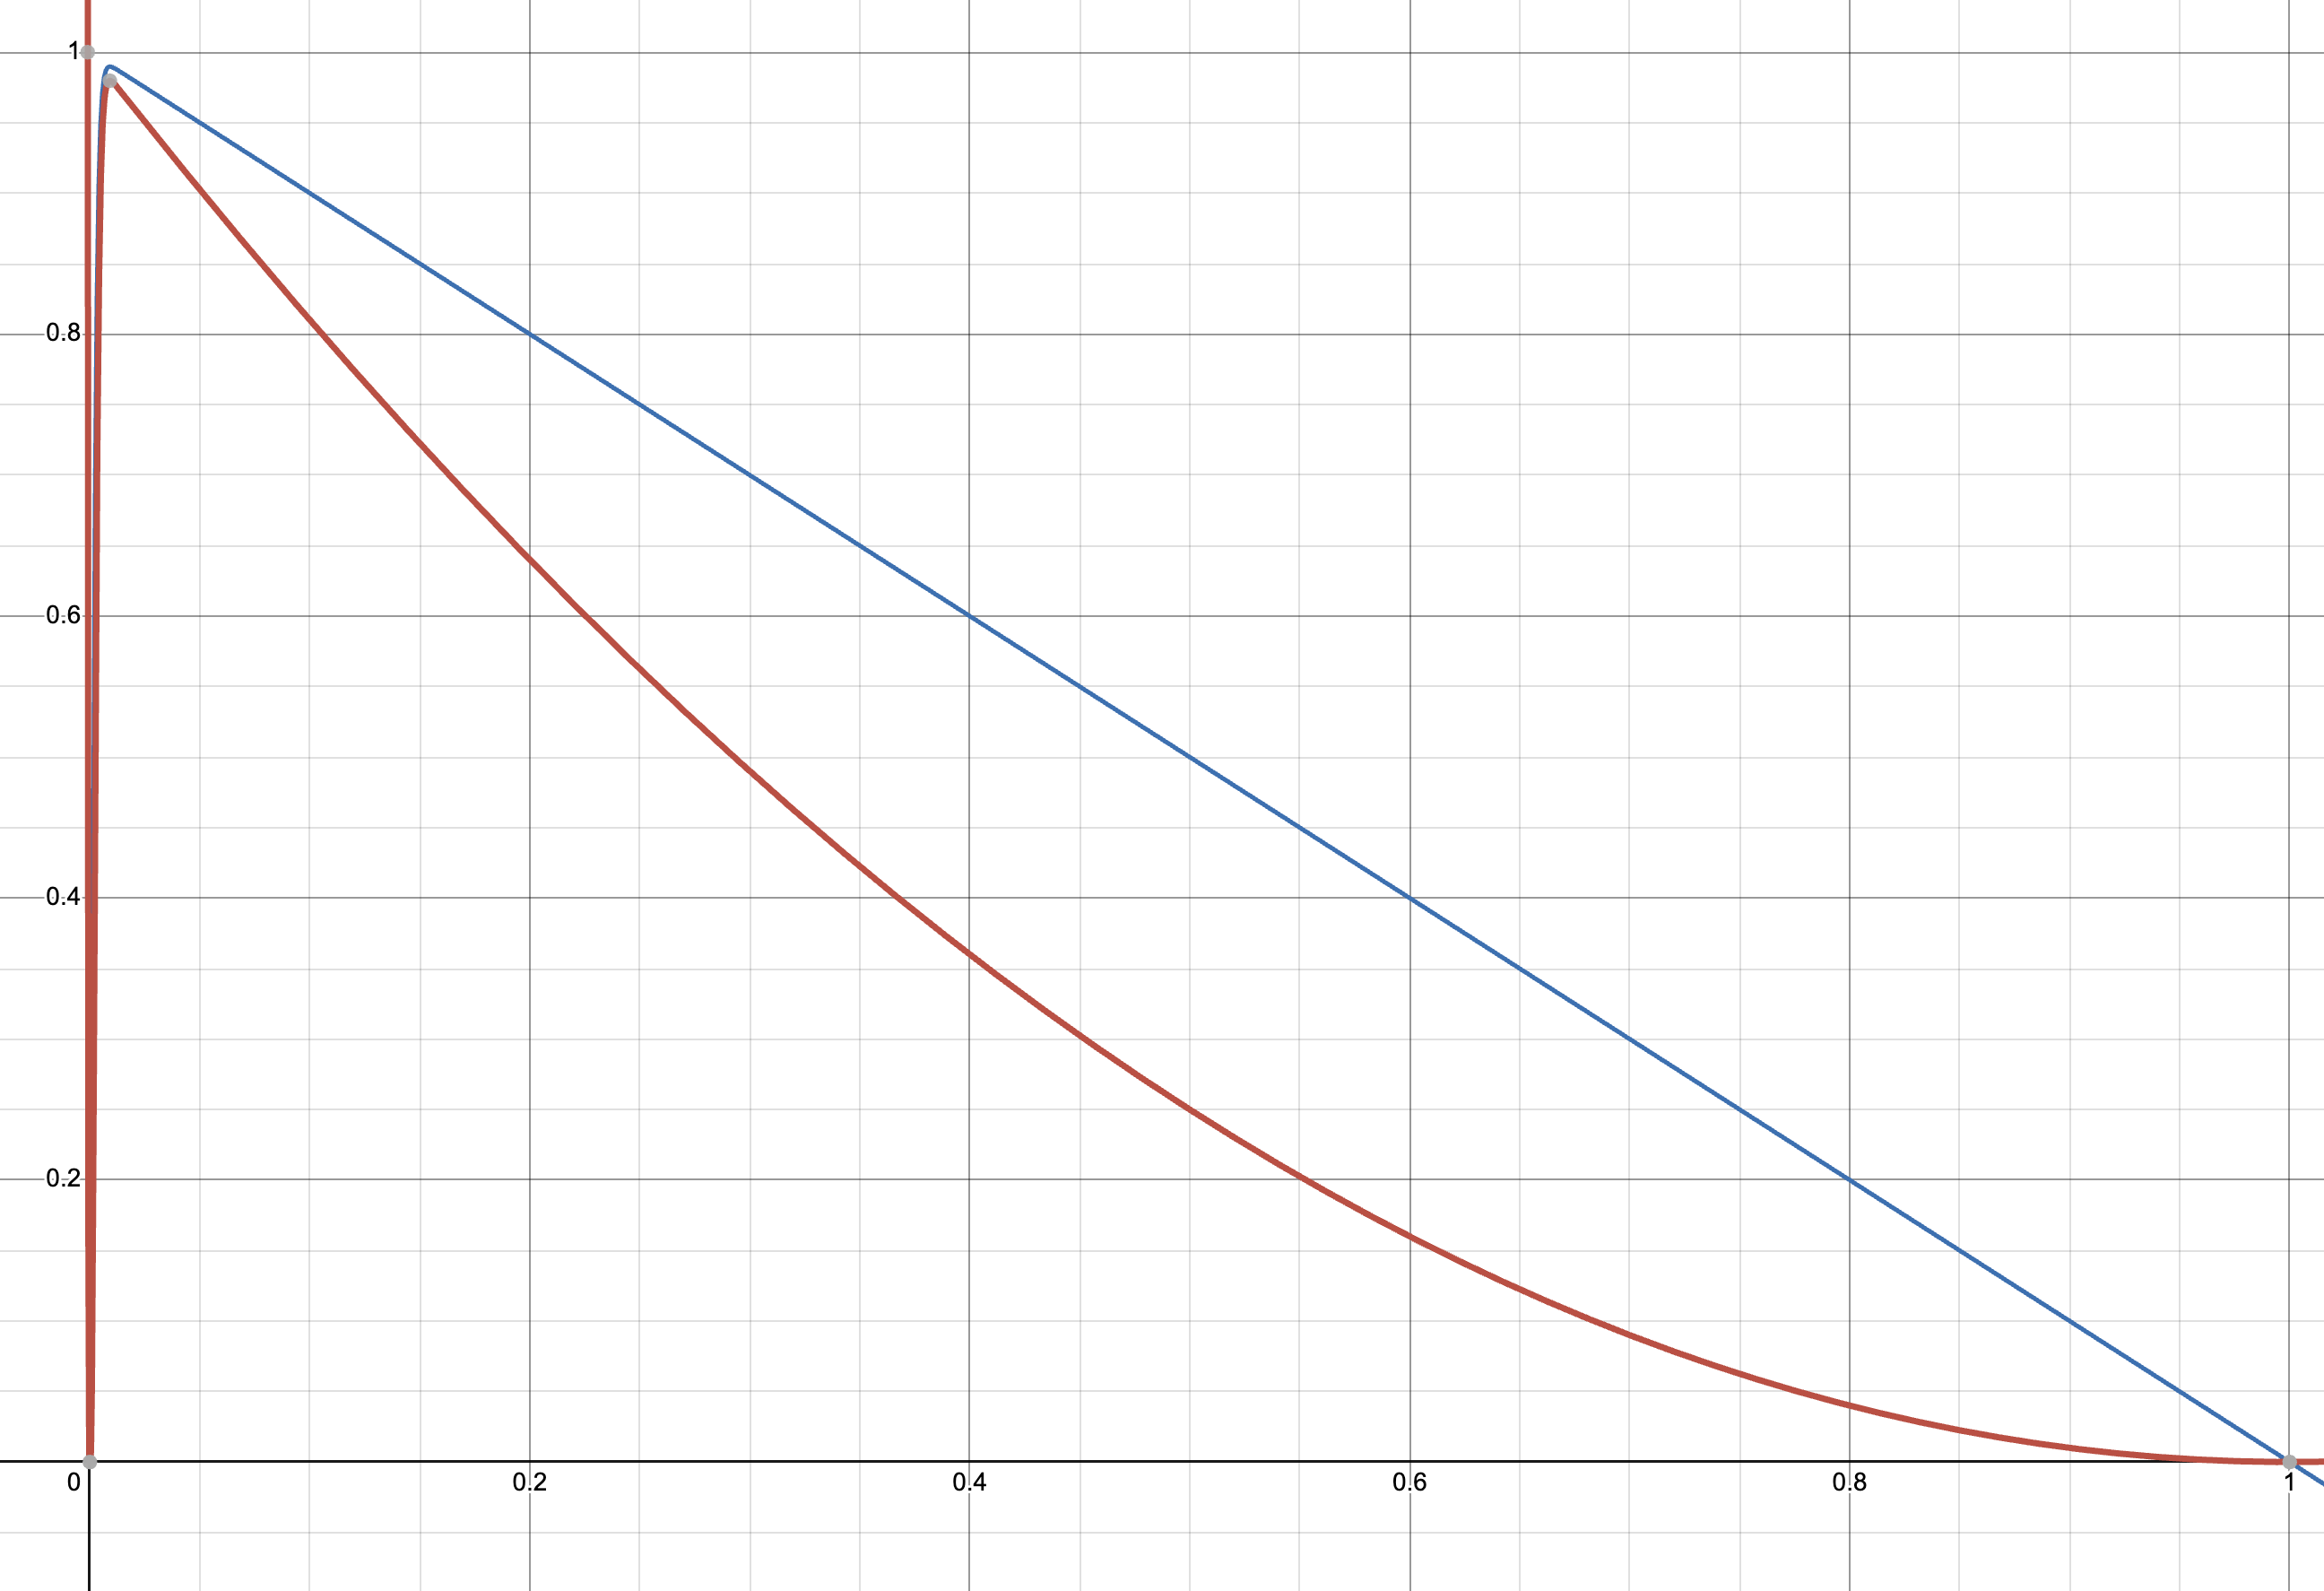
\includegraphics[width=0.75\linewidth]{pics/t=1,2.png}
  \end{figure}
\end{example}
Another observation is that when the random graph is not Erdos-Renyi, the inequality~\eqref{eq:z_it} depends on the selected vertices.
Thus, it is possible to dynamically adapt the bounds with respect to the selected vertices when computing value functions.
Also, for the non Erdos-Renyi case, we might replace $\prod_{j=1}^{t-1}(1-p_{iv_j})$ by
${m}_i^{t-1}$ where ${m}_i:=\left(\prod_{j\in N\setminus i}(1-p_{ij})\right)^{1/n}$ as an approximation.

For the way of efficiently selecting vertices or developing valid inequalities in the first stage might be done easily by primal-dual relaxations.
For example, in the authors' previous works, the first stage is guaranteed to be optimal by the strict complementarity of the primal-dual pair of the SDP relaxation. We expect similar results for this problem.

Suppose the inequality~\eqref{eq:z_it} is added to the LP relaxations above, we have
\begin{align*}
  \begin{split}
    \max\quad &\sum_{i\in N}w_i\sum_{t=1}^{n}z^t_i\\
    \text{ s.t.}\quad&z^t_i+z^t_j\leq 2-p_{ij},\quad\forall i,j\in N\\
    &z_i^t\leq (1-\gamma_i)^{t-1}{m}_i^{t-1}\\
    &0\leq z_i\leq 1,\quad \forall i\in N,
  \end{split}
\end{align*}
and its dual
\begin{align*}
  \min\quad &\sum_{t=1}^{n}\sum_{i\in N}(1-\gamma_i)^{t-1}{m}_i^{t-1}\lambda_{ii}+\sum_{t=1}^{n}\sum_{i,j\in N}(2-p_{ij})\lambda_{ij}\\
  \text{s.t.}\quad &\lambda^t_{ii}+\sum_{j\in N\setminus i}\lambda^t_{ij}\geq w_i,\quad \forall i\in N,t=1,\ldots,n\\
  &\lambda\geq 0.
\end{align*}
Thus when $S\subseteq N$ is given, we can consider the following value function approximation:
\[v(S):=\sum_{t=1}^{n}\left[\sum_{i\in S}(1-\gamma_i)^{t-1}{m}_i^{t-1}\lambda^t_{ii}+\sum_{\{i,j\}\subseteq S}(2-p_{ij})\lambda^t_{ij}+\sum_{i\in S,j\notin S}\lambda^t_{ij}\right],\]
and we have
\[v(S)-\E[v(S\setminus i\cup\delta_i)]\geq \sum_{t=1}^{n}\left[(1-\gamma_i)^{t-1}{m}_i^{t-1}\lambda^t_{ii}+\sum_{j\in N\setminus i}\lambda_{ij}^t\right]\geq \lambda_{ii}^1+\sum_{j\in N\setminus i}\lambda_{ij}^1\geq w_i.\]

Consider the following LP:
\begin{align*}
  \begin{split}
    \max\quad &\sum_{i\in N}w_i\sum_{t=1}^{n}x^t_i\\
    \text{ s.t. }
    &x_i^t\leq \left(1-\sum_{j=1}^{t-1}x_i^j\right)\prod_{j\in\Xi_i^t}(1-p_{ij}),\\
    &\sum_{i=1}^{n}x_i^t\leq1,\quad\forall t\\
    &\sum_{t=1}^{n}x_i^t\leq1,\quad\forall i\\
    &0\leq x^t_i,\quad \forall i\in N,
  \end{split}
\end{align*}
where $\Xi_i^t$ is the set of $j\in N\setminus\{i\}$ such that $p_{ij}$ is one of the $(t-1)$ smallest $p_{ik}$.
Denote the constraints as:
\begin{align}
  \label{eq:LP constraints}
  \begin{split}
    &x_i^t\leq \left(1-\sum_{j=1}^{t-1}x_i^j\right)\prod_{j\in\Xi_i^t}(1-p_{ij}),\\
    &\sum_{i=1}^{n}x_i^t\leq1,\quad\forall t\\
    &\sum_{t=1}^{n}x_i^t\leq1,\quad\forall i\\
    &0\leq x^t_i,\quad \forall i\in N,
  \end{split}
\end{align}

Go back to the previous inequality:
\begin{align*}
  \sum_{\tau=t}^n z_i^\tau\geq \Pr[i\text{ is isolated at stage }t]=&\sum_{S\subseteq N,|S|\leq N-(t-1),i\in S}\Pr[\text{State at $t$ is $S$}]*\Pr[i\text{ is isolated}|\text{state at $t$ is $S$}]\\
  =&\sum_{S\subseteq N,|S|\leq N-(t-1),i\in S}\sum_{T\subseteq N\setminus S,|T|=t-1}\prod_{j,k\in T,j\neq k}(1-p_{jk})\prod_{k\in N\setminus S\setminus T}(1-\prod_{j\in T}(1-p_{jk}))\prod_{j\in S\setminus\{i\}}(1-p_{ij})\\
  \geq &\max_{S\subseteq N,|S|\leq N-(t-1),i\in S}\Pr[\text{State at $t$ is $S$}]*\Pr[i\text{ is isolated}|\text{state at $t$ is $S$}]\\
  =&\max_{S\subseteq N,|S|\leq N-(t-1),i\in S}\sum_{T\subseteq N\setminus S,|T|=t-1}\prod_{j,k\in T,j\neq k}(1-p_{jk})\prod_{k\in N\setminus S\setminus T}(1-\prod_{j\in T}(1-p_{jk}))\prod_{j\in S\setminus\{i\}}(1-p_{ij})\\
  \geq &\max_{S\subseteq N,i\in S,|S|=n-(t-1)}\sum_{T=N\setminus S}\prod_{k\in T}\prod_{j\in T,j>k}(1-p_{jk})*1*\prod_{j\in S\setminus\{i\}}(1-p_{ij})\\
  &\text{OR}\\
  \geq &\max_{S=\{i\}}\sum_{T\subseteq N\setminus\{i\},|T|=t-1}\prod_{k\in T}\prod_{j\in T,j>k}(1-p_{jk})\prod_{k\in N\setminus\{i\}\setminus T}(1-\prod_{j\in T}(1-p_{jk}))
\end{align*}
where $p_{ii_1}\leq p_{ii_2}\leq\ldots\leq p_{ii_{n-1}}$.

Let $H$ be any set of the first $t-1$ selected vertices not including $i$, then
\[\Pr[\text{$i$ in the neighbor of $H$}]=\left(1-\prod_{j\in H}(1-p_{ij})\right)\]
while as an event, $i$ in the neighbor of $H$ implies that given $i$ is not selected during the first $t-1$ epochs, it cannot be selected in the later epochs, which is:
\[\Pr[\text{$i$ is not selected during $t,\ldots,n$}|\text{$i$ is not selected during $1,\ldots,t-1$}]\geq \left(1-\prod_{j\in H}(1-p_{ij})\right)\]
which implies
\begin{align*}
  \frac{\Pr[\text{$i$ not selected}]}{\Pr[\text{$i$ not selected in $1,\ldots,t-1$}]}&\geq\left(1-\prod_{j\in H}(1-p_{ij})\right)\\
  \frac{1-\sum_{\tau=1}^{n}x_i^t}{1-\sum_{\tau=1}^{t-1}x_i^\tau}&\geq \left(1-\prod_{j\in H}(1-p_{ij})\right)\\
  \sum_{\tau=t}^{n}x_i^\tau&\leq \prod_{j\in H}(1-p_{ij})\left(1-\sum_{\tau=1}^{t-1}x_i^\tau\right).
\end{align*}
Thus, we can consider the relaxation:
\begin{align*}
  \begin{split}
    \max\quad &\sum_{i\in N}w_i\sum_{t=1}^{n}x^t_i\\
    \text{ s.t. }
    &x_i^t\leq \left(1-\sum_{j=1}^{t-1}x_i^j\right)\prod_{j\in H}(1-p_{ij}),\\
    &\sum_{\tau=t}^{n}x_i^\tau\leq \prod_{j\in H}(1-p_{ij})\left(1-\sum_{\tau=1}^{t-1}x_i^\tau\right)\\
    &\sum_{i=1}^{n}x_i^t\leq1,\quad\forall t\\
    &\sum_{t=1}^{n}x_i^t\leq1,\quad\forall i\\
    &0\leq x^t_i,\quad \forall i\in N.
  \end{split}
\end{align*}
In practice, the $H$ on the RHS of the inequality should be replaced by a known set of vertices, say $\Xi_i^t$ for the first inequality.
However, we conjecture that these inequalities are facet-defining, since when both $n$ and $p$ get large, the optimal value of the relaxation seems to be converging to the optimal DNP value for $G(n,p)$.

\rgnote{Check this result later} Notice that for any epoch $t$, the probability of not selecting any vertex at $t$ is equivalent to there is no vertex to select (i.e., the graph is empty).
Thus, at time $t$, let $H$ be the set of selected vertices, we have
\begin{align*}
  &\Pr[\text{not select any vertex at $t$}|\text{$H$ is selected during $1,\ldots,t-1$}]\\
  =&\Pr[\text{all vertices in $N\setminus H$ are in the neighbor of $H$}]\\
  =&\prod_{j\in N\setminus H}\left(1-\prod_{k\in H}(1-p_{ij})\right)\\
  =&\frac{\Pr[\text{no vertex selected at $t$, $H$ is selected during $1,\ldots,t-1$}]}{\Pr[\text{$H$ is selected during $1,\ldots,t-1$} ]}
\end{align*}
By summing over all possible $H\subseteq N$ with $|H|\leq t-1$ (not $|H|=t-1$ cuz it is not guaranteed that a vertex was selected during all $1,\ldots,t-1$), we get
\begin{align*}
  &\sum_{H\subseteq N,|H|\leq t-1}\Pr[\text{no vertex selected at $t$}, \text{$H$ is selected during $[t-1]$}]\\
  =&\sum_{H\subseteq N,|H|\leq t-1}\Pr[N\setminus H\text{ is in the neighbor of $H$}]*\Pr[\text{$H$ is selected during $[t-1]$}]\\
  (\iff)&\\
  &1-\sum_{i=1}^{n}x_i^t\\
  =&\sum_{H\subseteq N,|H|\leq t-1}\prod_{j\in N\setminus H}\left(1-\prod_{k\in H}(1-p_{ij})\right)\Pr[\text{$H$ is selected during $[t-1]$}]
\end{align*}
% \[\sum_{i=1}^{n}x_i^t=\prod_{j\in N\setminus H}\left(1-\prod_{k\in H}(1-p_{ij})\right)\]
An easy inequality is for $t\leq \tau$
\[\sum_{i=1}^{n}x_i^t\geq\sum_{i=1}^{n}x_i^\tau\]
Also,
\[1-\sum_{i=1}^{n}x_i^t=\Pr[\text{graph is empty at time $t$}]\]
Consider $\beta^t:=\Pr[\text{the graph is not empty at $t-1$ but empty at $t$}]=\Pr[\text{the graph becomes empty after $t-1$th vertex is chosen}]$.
Then let $G^t$ be the graph at the beginning of epoch $t$, e.g. $G^1=G$, notice all $G^t$ are random graphs with edges not realized yet.
\[1-\sum_{i=1}^{n}x_i^t=\Pr[G^t=\emptyset,G^{t-1}=\emptyset]+\beta^t=\Pr[G^{t-1}=\emptyset]+\beta^t=\Pr[G^1=\emptyset]+\sum_{\tau=2}^{t}\beta^\tau=\sum_{\tau=2}^{t}\beta^\tau\]
Also, we can have
\[\Pr[G^t=\emptyset|G^{t-1}\neq\emptyset]=1-\frac{\sum_{i=1}^{n}x_i^t}{\sum_{i=1}^{n}x_i^{t-1}}.\]
Similarly, we can have
\begin{align*}
  \sum_{i=1}^{n}x_i^t&=\Pr[\text{a vertex chosen at }t]\\
  &=\Pr[G^t\neq\emptyset]\\
  &=\sum_{H\subseteq N,|H|=t-1}\Pr[\text{not all $i\in N\setminus H$ in the neighbor of $H$}|\text{$H$ is chosen in }1,\ldots,t-1]\Pr[\text{$H$ is chosen in }1,\ldots,t-1]\\
  &=\sum_{H\subseteq N,|H|=t-1}(1-(\prod_{i\in N\setminus H}(1-\prod_{j\in H}q_{ij})))\Pr[\text{$H$ is chosen in }1,\ldots,t-1]\\
  &\leq \max_{H\subseteq N,|H|=t-1}(1-(\prod_{i\in N\setminus H}(1-\prod_{j\in H}q_{ij})))
\end{align*}
\rgnote{Note that $\sum_{\tau=t}^{n}\sum_{i=1}^{n}x_i^\tau$ does not represent the probability of a vertex being selected during $t,\ldots,n$ because the events "a vertex selected at $t$" and "a vertex is selected at $t+1$" are not exclusive. But it does represent the expected number of vertices selected during $t,\ldots, n$.
However, $\sum_{i=1}^n x_i^\tau$ represents the probability of selecting a vertex in $t,\ldots,n$ as well}
We might be able to get a nest sum of graph being empty at some epoch $t$.
\[1 >= \Pr[\text{graph is empty between epoch $2$ and $n$}]=\]
\section{Compute $x_i^t$ for $G(n,p)$}
Consider $G(n,p)$ where the greedy policy is optimal, and assume $w_1\geq w_2\geq \ldots\geq w_n$, then by assuming $j_1=1,j_t=i$, $x_i^t$ can be exactly expressed as:
\begin{align}
  \begin{split}
    x_i^t=&\sum_{j_2=2}^{i-(t-2)}\sum_{j_3=j_2+1}^{i-(t-3)} \sum_{j_4=j_3+1}^{i-(t-4)}\ldots\sum_{j_{t-1}=j_{t-2}+1}^{i-1}\left[p^{j_2-1-1}(1-p)\right]\left[(1-(1-p)^2)^{j_3-j_2-1}(1-p)^2\right]\ldots\left[(1-(1-p)^{t-2})^{j_{t-1}-j_{t-2}-1}(1-p)^{t-2}\right]\\
    &*\left[(1-(1-p)^{t-1})^{i-j_{t-1}-1}(1-p)^{t-1}\right]\\
    =&q^{t(t-1)/2}\prod_{k=1}^{t-1}(1-q^k)^{-1}\sum_{j_2=2}^{i-(t-2)}\sum_{j_3=j_2+1}^{i-(t-3)} \sum_{j_4=j_3+1}^{i-(t-4)}\ldots\sum_{j_{t-1}=j_{t-2}+1}^{i-1}(1-q^{1})^{j_2-j_1}(1-q^{2})^{j_3-j_2}\ldots(1-q^{t-1})^{j_t-j_{t-1}}  \\
    =&q^{(t-1)t/2}\prod_{k=1}^{t-1}(1-q^k)^{-1}\sum_{j_2=2}^{i-(t-2)}\sum_{j_3=j_2+1}^{i-(t-3)} \sum_{j_4=j_3+1}^{i-(t-4)}\ldots\sum_{j_{t-1}=j_{t-2}+1}^{i-1}\frac{(1-q^{t-1})^{j_t}}{(1-q^1)^{j_1}}\left(\frac{1-q^1}{1-q^2}\right)^{j_2}\left(\frac{1-q^2}{1-q^3}\right)^{j_3}\ldots \left(\frac{1-q^{t-2}}{1-q^{t-1}}\right)^{j_{t-1}}
  \end{split}
\end{align}
and
\[x_i^t=0,\forall t>i.\]
It is not hard to see that when $j_2,j_3,\ldots,j_{t-1}$ are fixed, the product term represents the probability of the policy selecting $1$ at $t=1$, $j_k$ at time $k$ and $i$ at time $t$.

Some valid inequalities hence can be obtained by the formulation above:
\begin{align*}
  &(1-q)^{i-1}{i-2\choose t-2}q^{t(t-1)/2}\prod_{k=1}^t(1-q^k)^{-1}\\
  \leq &x_i^t\\
  \leq &(1-q^{t-1})^{i-1}{i-2\choose t-2}q^{t(t-1)/2}\prod_{k=1}^t(1-q^k)^{-1}
\end{align*}

This works for greedy policy on general graphs.

Another generalization is that the probability of selecting a vertex at time $t$ is at least the probability that there is still a vertex left at time $t$.

\section{Lassere Hierarchy}
Consider a Lasserre hierarchy similar to the one in the paper by Cifuentes, Shu, Toriello.
Consider the power set $2^{n^2}$ of $\{(i,t):i,t\in[n]\}$, and define
\[v_T=\left(\mathbbm{1}\{S\subseteq T\}\right)_{S\subseteq 2^{n^2}}\in 2^{n^2}.\]
Fix an arbitrary optimal policy of the problem, and let $q_S$ be the probability that $S\subseteq [n]\times [n]$ is picked under this policy.
For example, if $S=\{(1,1),(2,3),(5,4)\}$, $q_S$ is the probability that $1$ is picked at time $1$, $2$ picked at time $3$ and $5$ picked at time $4$ under this policy.
Then we have this SDP:
\begin{align*}
  \psi_t(y)=\max_{y\in 2^{n^2}}~&\sum_{i=1}^{n}\sum_{t=1}^{n}y_{(i,t)}\\
  \text{s.t.}~&y_\emptyset=1\\
  &0\leq y_S\leq q_S,\forall S\subseteq [n]\times[n], |S|\leq 2t\\
  &M_t(y)\succeq 0
\end{align*}
\begin{theorem}
  The hierarchy defined above satisfies
  \[\E[\hat{\alpha}(G)]= \psi_n(y)\leq\ldots\leq \psi_1(y),\]
  where $\E[\hat{\alpha}(G)]$ denotes the expected size of the stable set returned by an optimal policy, i.e., the optimal value of the optimal policy.
\end{theorem}
\begin{proof}
  The proof is similar to the one in the paper by Cifuentes, Shu, Toriello.
  
  First, sample a $T$ returned by the optimal policy.\rgnote{Need more details}.
  Define $\hat{y}$ such that $\hat{y}_S$ represents the probability that $S\subseteq T$.
  We claim that $\hat{y}$ is feasible for $\psi_n(y)$, and its objective value is exactly $\E[\hat{\alpha}(G)]$.

  First $\hat{y}_{\emptyset}=1$ clearly, and $\hat{y}_S\geq 0$ for every $S\subseteq [n]\times[n]$. Since $T$ is return by the optimal policy, we have 
  \[\hat{y}_S=\Pr[S\subseteq T]\leq\Pr[S\text{ is picked under this policy}]=q_S.\]
  For each $T'\subseteq 2^{n^2}$, we defined $v_{T'}$ such that $[v_{T'}]_S=\mathbbm{1}_{S\subseteq T'}$. Then by the definition of $\hat{y}$, we have 
  \[\hat{y}=\sum_{T'\subseteq[n]\times[n]}\Pr[T'=T]v_{T'}.\]
Thus, $\hat{y}\in\conv\{v_{T'}:T'\subseteq[n]\times[n]\}$, and the fact that $M_n^n(y)\succeq 0$ follows from the fact that the Lasserre hierarchy at the last level equal to the convex hull of the projection.
Thus, $\hat{y}$ is feaisble for the SDP.
Since $\hat{y}_{(i,t)}$ is the probability that $i$ is selected at time $t$, we have 
\[\E[\hat{\alpha}(G)]=\E[\sum_{(i,t)\in[n]\times[n]}\mathbbm{1}\{(i,t)\in T\}]=\sum_{(i,t)\in [n]\times[n]}\hat{{y}}_{(i,t)}\]

Now we consider the other direction of the equality. Consider any feasible solution $y$ of the SDP. $y_{(i,t)}\leq q_{(i,t)}$ for every $(i,t)\in[n]\times[n]$, and hence 
\[\sum_{(i,t)\in[n]\times[n]}y_{(i,t)}\leq \sum_{(i,t)\in[n]\times[n]}q_{(i,t)}=\E[\hat{\alpha}(G)].\]


  The inequalities are due to the fact that as the level of hierarchy increases, the feasible set becomes smaller.
\end{proof}
However, without knowing the optimal policy, it is hard to compute the value of the SDP. Even if we know, computing the $q_S$ is still expensive in general, an example can be seen when the graph is Erdos-Renyi, where the greedy algorithm is optimal.

Thus, we can only try to provide upper bounds for $q_S$ for each level of relaxations.
\rgnote{We expect the first level hierarchy to be good enough in practice. In fact, while the LP relaxation performs well in many cases, the first level hierarchy considers the interaction $\Pr[\text{$i$ selected at $t$ and $j$ selected at $\tau$}]$, which should bring more information because no interaction is considered in the LP relaxation.}

In fact, since for any $(i,t)$, $(j,\tau)$, if $i=j$, $t\neq\tau$, then $\Pr[(i,t),(j,\tau)]$ is $0$. Similarly, if $t=\tau$, $i\neq j$, $\Pr[(i,t),(j,\tau)]$ is $0$.
Thus, in total, there are at most $(n-1)^2n^2/2+n^2$ non-zero entries in the moment matrix, which is in $O(n^4)$.

With respect to this SDP model, which is large in general, we might still be able to bound each entry.
Also, according to the numerical experiments, the $y_{(i,t)}$ when $t$ gets large is approaching $0$.
Thus, when we are actually solving the SDP, we might be able to ignore some of the variables to reduce the dimension.

For example, when we consider the probability of $i$ being selected before $j$, then we should consider 
\[\sum_{t=1}^{n-1}\sum_{\tau=t+1}^{n}y_{(i,t),(j,\tau)}\leq \sum_{t=1}^{n-1}\prod_{k\in\Xi_{ij}^{t}}(1-p_{jk})\sum_{\tau=1}^{t}y_{(i,\tau)}\]
where $\Xi_{ij}^{t}:=\argmax_{H\subseteq N, |H|=t, i\in H,j\notin H}\prod_{k\in H}(1-p_{jk})$.
Similarly, consider 
\[\Pr[\text{$i$ selected at $t$}|\text{$j$ selected at $\tau$}]\leq \prod_{k\in \Xi_{i,j}^{t,\tau}}(1-p_{ik})(1-p_{jk})\]
which is equivalent to 
\[y_{(i,t),(j,\tau)}\leq \prod_{k\in \Xi_{i,j}^{t,\tau}}(1-p_{ik})(1-p_{jk})y_{(j,\tau)}\]

The probability of selecting vertex $i$ at time $t$ can be fully described by the previous actions and $t+1$ actions.

Notice that selecting a vertex $i$ at time $t$ implies that a vertex is selected at each $1,\ldots, t-1$. 
Thus, we can consider the following equality:
\[y_{(i,t),(i,t)}=\sum_{j=1}^{n}y_{(i,t),(j,\tau)}\forall 1\leq \tau\leq t-1.\]
Similarly, selecting $i$ at time $t$ is equivalent to selecting $i$ at time $t$ and a vertex at time $t+1$ or selecting $i$ at time $t$ and no vertex left at time $t+1$.
Thus, we have the following equality:
\[y_{(i,t),(i,t)}=\sum_{j=1}^{n}y_{(i,t),(j,t+1)}+\Pr[G^{t+1}=\emptyset,i\text{ selected at }t]\]
In general, we are not able to compute the second term due the fact that it requires knowing the probability of $G^t$ reaching a certain state. 
However, to bound such a term, it might be helpful to consider the expected number of vertices discarded at time $t$, equivalently, the expected number of remaining vertices at time $t$.

Overall, the SDP we are trying to solve is:
\begin{align*}
  \max\quad&\sum_{t=1}^{n}\sum_{i=1}^{n}x_i^t\\
  &\begin{bmatrix}
    1&x^\top \\
    x&X
  \end{bmatrix}\succeq 0\\
  &X\geq 0\\
  &\diag(X) = x\\
  &X_{(i,n),(j,t)}\leq \prod_{k\neq j}1-p_{jk},\quad\forall i,j,t\\
  &x_{i}^{t} = \sum_{j\neq i}X_{(i,t),(j,\tau)},\quad\forall \tau<t\\
  &x_{i}^{t} \geq \sum_{j\neq i}X_{(i,t),(j,\tau)},\quad\forall \tau>t\\
  &x_i^1 = \sum_{j\neq i}X_{(i,1),(j,2)} + \left(\prod_{j\neq i}p_{ij}\right)x_i^1,\quad \forall i\\
  &\sum_{i=1}^{n}x_i^1 = 1\\
  &\sum_{i=1}^{n}x_i^t \leq 1,\quad \forall t\geq 2\\
  & X_{(i,t),(i,\tau)} = 0,\quad\forall t\neq \tau\\
  & X_{(i,t),(j,t)} = 0,\quad\forall i\neq j\\
  &\sum_{i=1}^{n}x_i^t \leq \max_{H\subseteq N,|H|=t-1}\left[1-\left(\prod_{j\notin H}\left(1-\prod_{k\in H}(1-p_{jk})\right)\right)\right],\quad \forall t\geq 2\\ %\prod_{j\neq k\in H}(1-p_{jk})
  &X_{(i,t),(j,\tau)}\leq x_i^t~\max_{H\subseteq H\setminus\{i,j\},|H|=\tau-t-1}\prod_{k\in H}(1-p_{ik})(1-p_{jk}),\quad\forall i,j,t<\tau\\
  &\sum_{\tau=t}^{n}x_i^\tau\leq \max_{H\subseteq N\setminus\{i\},|H|=t-1}\prod_{j\in H}(1-p_{ij})\left(1-\sum_{\tau=1}^{t-1}x_i^\tau\right),\quad \forall i,t\\
  &\sum_{t=1}^{n-1}\sum_{\tau=t+1}^{n}X_{(i,t),(j,\tau)}\leq \sum_{t=1}^{n-1}\prod_{k\in\Xi_{ij}^{t}}(1-p_{jk})\sum_{\tau=1}^{t}x_i^\tau,\quad\forall i,j\\ %# TODO: Check this equation, it seems like we calculate some probability many times because Xi_{ij}^t does not catch the probability $i$ is selected at $t$ but during 1,..,t 
  &\sum_{t=1}^{n-1}\sum_{\tau=t+1}^{n}X_{(i,t),(j,\tau)}+\sum_{t=1}^{n-1}\sum_{\tau=t+1}^{n}X_{(j,t),(i,\tau)}\leq (1-p_{ij})\min\left(\sum_{t=1}^{n}x_i^t,\sum_{t=1}^{n}x_j^t\right)
\end{align*}

This optimization problem is a relaxation of the DNP problem.
Consider an arbitrary policy $\mathcal{P}$ for the problem,
Let $v = [1~X_1^1~\ldots~X_n^n]^\top$ where $X_i^t$ is the random Bernoulli variable indicating vertex $i$ is selected at time $t$ under policy $\mathcal{P}$.
Consider $Y:=\E[vv^\top]$, it is not hard to see that $a^\top Ya=\E[a^\top vv^\top a]\geq 0$ for any $a\in\R^{n^2+1}$ 
by the linearity of expectation.
Thus, $Y$ is positive semidefinite.
In particular, $Y_{(i,t)}=\Pr[(X_i^t)^2 = 1]=\Pr[X_i^t = 1]$;
$Y_{(i,t),(j,\tau)} = \Pr[X_i^tX_j^\tau = 1] = \Pr[X_i^t = 1, X_j^\tau = 1]$.
It is clear that $Y$ satisfies all constraints of the SDP above because all the constraints are upper bound on 
$\Pr_{\mathcal{P}}[X_i^t=1], \Pr_{\mathcal{P}}[X_i^t=1,X_j^\tau =1]$.

For the first $2$ epochs, the $\sum_{i=1}^{n}x_i^1,\sum_{i=1}^{n}x_i^2$ are tight. 
Note $\sum_{i=1}^{n}x_i^1 = 1$ and $\sum_{i=1}^{n}x_i^2 = 1-\sum_{i}\prod_{j\neq i}p_{ij} x_i^1 = 1 - \Pr[G^2=\emptyset].$

\emph{Conjecture 1:} For $G(n,p)$, $x_i^1$ is an optimal policy for stage $1$. According to the experiments, when the weights are equal, $x_i^1 = 1/n$ is returned; otherwise, $x_i^t = 1$ if $i$ is the vertex with largest weight.
If $i,j$ both the same largest weight, then $x_i^1 = x_j^1 = 1/2$.

\emph{Conjecture 2:} For general instances, the accuracy of $x_i^1$ depends on the variance of $p_{ij}$ (or possibly $\max p_{ij} - \min p_{ij}$).
% \[\max_{H\subseteq N,|H|=n-t,i\notin H}\prod_{j\in H}p_{ij}\]
\subsection{Previous Lasserre Hierarchy Idea}
Consider an arbitrary optimal policy of the stochastic maximum stable set problem.
Let $\{(S^*,T^*)\}$ denote a random sequence of vertices selected by the optimal policy.
The sequence looks like $\{(i_1,1),(i_2,2),(i_3,3),\ldots, (\emptyset, t),\ldots,(\emptyset,n)\}$, where $(\emptyset,t)$ represents that the graph is already empty at time $t$ so no vertex to select.
Note that since this is a sequence, for every $i\in V$, there is no $t\neq \tau$ such that $(i,t),(i,\tau)\in \{(S^*,T^*)\}$; for any $t\in[n]$, there is no $j\neq j\in V$ such that $(i,t),(j,t)\in\{(S^*,T^*)\}$.
Also, $\E[|S^*|]$ is the expected size of the stable set returned by an optimal policy. That is, it is the optimal value of the value function evaluation LP.

Denote $X_i^t\in\{0,1\}$ as a random indicator variable that the vertex $i$ is selected by the optimal policy at time $t$.
With respect to our previous model, $\Pr[X_i^t=1]=x_i^t$.
Now we consider the Lassere hierarchy corresponding to~\eqref{eq:LP constraints}.
Due to expensive computational costs, we only consider the moment matrix without including slack moment matrices.
\begin{align*}
  \begin{split}
    \max\quad &\sum_{i=1}^{n}\sum_{t=1}^{n}y^t_i\\
    \text{s.t.}\quad &y_{\emptyset}^{\emptyset}=1\\
    &y_i^t\text{ satisfies~\eqref{eq:LP constraints}},\forall t,i\\
    &M_t(y)\succeq 0
  \end{split}
\end{align*}
where $M_t(y)$ represents the $t$-th moment matrix of $y$.
The SDP can be constrainted further, let $p_{(I,T)}$ be the probability that $(I,T)\subseteq (S^*,T^*)$, that is, it is the probability that for each $(i,t)\in (I,T)$, $i$ is selected by the optimal policy at time $t$.
Then we have
\begin{align*}
  \begin{split}
    \max\quad &\sum_{i=1}^{n}\sum_{t=1}^{n}y^t_i\\
    \text{s.t.}\quad &y_{\emptyset}^{\emptyset}=1\\
    &y_i^t\text{ satisfies~\eqref{eq:LP constraints}},\forall t,i\\
    &y_I^T\leq p_I^T,\forall |I|,|T|\leq t\\
    &M_t(y)\succeq 0
  \end{split}
\end{align*}
Then let $\hat{y}\in\R^{n^2}$ be the probability that the random $(S^*,T^*)$ contains $(I,T)$ as a subsequence.
Clearly, $\hat{y}_{\emptyset}=1$ and $\hat{y}\geq 0$.
Also,
\[\hat{y}_I^T=\Pr[(I,T)\subseteq (S^*,T^*)]=p_I^T.\]
Also, if we let $u_{J,\tau}\in\R^{2^{n^2}}$ where $(u_{S,\tau})_{I,T}=\mathbbm{1}_{(S,\tau)\supseteq (I,T)}$.
Then $\hat{y}=\sum_{(S,\tau)}\Pr[(S^*,T^*)=(S,\tau)]u_{(S,\tau)}$.
So $\hat{y}\in\conv\{u_{(S,\tau)}\}$ and hence $M_{n^2}(y)\succeq 0$. So $\hat{y}$ is feasible for the $n^2$-th hierarchy.
As before, $\E[|S^*|]=\sum\hat{y}_i^t$.

In addition, it is not hard to see that $\hat{y}_i^t$ satisfied~\eqref{eq:LP constraints}.

Then the problem becomes: how to compute $p_I^T$ or closely approximate it.
While computing $p_I^T$ is almost equivalent to solve the problem, it might be more reasonable to do an estimation.
A clear upper bound of $p_I^T$ is the probability of $I$ being independent, which brings us to the SDP relaxation given by Kevin, Cifuentes and Toriello.
In practice, it might be sufficient to just consider the second level hierarchy.

\section{SDP Relaxation based on Lov\'asz Theta Function}
Consider the previous SDP in the the paper by Diego Cifuentes, Kevin Shu and Alejandro Toriello:
\begin{align}
  \label{SDP-P'}
  \tag{SDP-P'}
  \begin{split}
    \max_{x,X}\quad &w^\top x\\
    \text{s.t.}\quad &0\leq X^t_{ij}\leq 1-p_{ij},\forall ij\in{n\choose{2}}\\
    &X^t_{ii}=x_i^t\\
    &x_i^t\leq (1-\sum_{j=1}^{t-1}x_i^j)\prod_{j=1}^{t-1}(1-p_{iv_j})\\
    &
    \begin{pmatrix}
      1&x^\top\\
      x&X
    \end{pmatrix}\succeq 0
  \end{split}
\end{align}
where $x\in\R^{n^2}$, $X\in\symm^{n^2}$.
Notice that $X_{ij}^t$ can be integer
Also, $X$ is a block diagonal matrix which is made of $n$ of matrices in $\symm^{n}$.
And its dual can be written as
\begin{align}
  \tag{SDP-D'}
  \begin{split}
    \min\quad &\alpha+\sum_t\sum v_{ij}^t(1-p_{ij})+\sum v^t_i(1-\gamma_i)^{t-1}m_i^{t-1}\\
    &q^t_i=-\frac{1}{2}u_i^t\\
    &Q^t_{ij}=\frac{v_{ij}^t-u_{ij}^t  }{2}\\
    &Q^t_{ii}=u_{i}^t+v_i^t-w_i\\
    &
    \begin{pmatrix}
      \alpha&q^\top\\
      q&Q
    \end{pmatrix}\succeq 0\\
    &u_{ij}^t\geq0\\
    &v^t\geq 0
  \end{split}
\end{align}
Thus, when $Q_{ij}^t>0$, to minimize $v_{ij}^t$, have $v_{ij}^t=Q_{ij}^t*2$; when $Q_{ij}^t\leq 0$, have $v_{ij}^t=0$.
Similar arguments apply to $v_i^t$, suppose $u_{i}^t, v_i^t>0$, then by setting $v_i^t=0$, there is an improvement. If $u_i^t\leq 0$, then making $v_i^t=Q_{ii}^t+w_i$ improves the objective value. Notice that since $q_i=-u_i^t/2 $, it is not necessary that we can always set $u_i^t=Q_{ii}^t+w_i$ and keep the matrix PSD.
That is, we can write the dual problem as:
\begin{align}
  \label{SDP-D'}
  \tag{SDP-D'}
  \begin{split}
    \min\quad &\alpha+\sum_t\sum [2Q_{ij}^t]^+(1-p_{ij})+\sum (Q_{ii}^t+w_i+2q_i^t)(1-\gamma_i)^{t-1}m_i^{t-1}\\
    &q^t_i=-\frac{1}{2}u_i^t\\
    &Q^t_{ij}=\frac{v_{ij}^t-u_{ij}^t  }{2}\\
    &Q^t_{ii}=u_{i}^t+v_i^t-w_i\\
    &
    \begin{pmatrix}
      \alpha&q^\top\\
      q&Q
    \end{pmatrix}\succeq 0\\
    &u_{ij}^t\geq0\\
    &v^t\geq 0
  \end{split}
\end{align}
\newpage
\bibliographystyle{splncs04}
\bibliography{SDPVFA}
\end{document}
